%\documentclass{article}
%\usepackage{graphicx,subfigure}
%\begin{document}

\begin{figure}[!h]
  \centering
  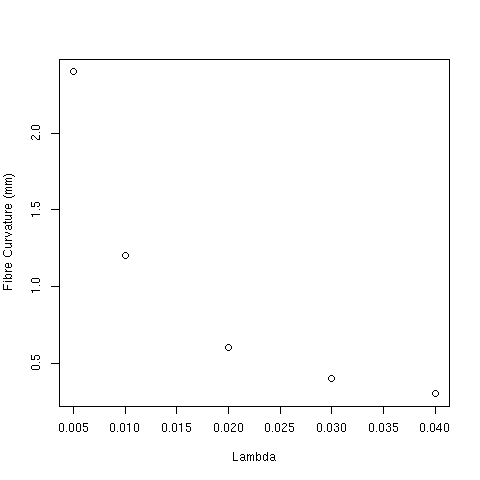
\includegraphics[width=0.9\textwidth]{curvlambda.png}
  \caption{Plot of fibre curvature calculated using equation~\ref{eqn:timowool} against $\lambda$ , with the other parameters held constant at $D=18$, $m=1$,$n=1$.}
  \label{fig:curvlambda}
\end{figure}

%\end{document}

